\chapter{Background}\label{cha:background}
This chapter covers the main theoretical concepts underlying the problem domain and proposed solution.
Section~\ref{sec:back-pollen} gives a short overview of the current methods that are in use for pollen counting and the data that is available. Based on this, Section~\ref{sec:back-problem} formalizes the task as a machine learning problem.
A theoretical overview of the main building blocks of modern convolutional neural networks follows in Section~\ref{sec:back-cnn}, together with an overview of the metrics used to measure the performance of object detection models in Section~\ref{sec:back-metrics}.
A basic understanding of the operation and components of a standard feedforward fully connected neural network is assumed for this section.

\section{Pollen Imaging}\label{sec:back-pollen}
There are two main methods of pollen analysis, image-based and non-image-based.
Non-image-based techniques employ a host of alternative sensing methods and will not be discussed further in this thesis.
Within the image-based methods there are two main imaging techniques.

\textit{Light microscopy} (LM) describes the method of observing a prepared sample with an optical microscope using visible light.
The sample is fixed to a translucent slide and is illuminated with a backlight.
It can either be observed through an eyepiece or photographed with an image sensor.
An example of a pollen grain is shown in Figure~\ref{fig:lm_and_sem}.
Because the grain is semi-translucent, differences in the surface texture can be observed, but only some areas are in focus.
A consequence of the high magnification is that the plane of focus is so narrow that only parts of the grain are in focus.

\begin{figure}[htb]
  \centering
  \begin{subfigure}[t]{0.4\textwidth}
    \centering
    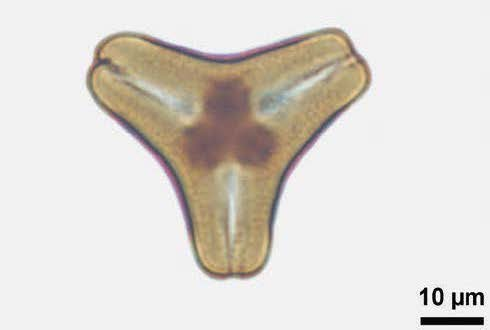
\includegraphics[width=\textwidth]{figs/background/pollen_lm.jpg}
    \caption{Light Microscopy}
  \end{subfigure}%
  \hspace*{0.04\textwidth}
  \begin{subfigure}[t]{0.4\textwidth}
    \centering
    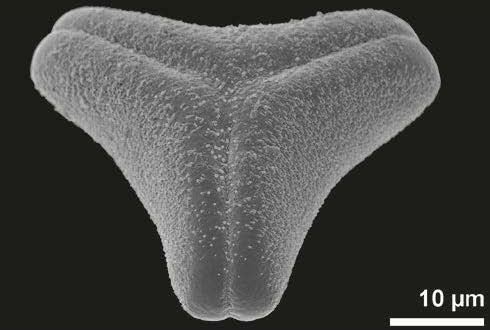
\includegraphics[width=\textwidth]{figs/background/pollen_sem.jpg}
    \caption{Scanning Electron Microscopy}
  \end{subfigure}
  \caption[Pollen grain imaging examples using LM and SEM]{\textit{Aetanthus coriaceus}.
  Imaged with LM (a) and SEM (b). \textcite[98]{halbritter_methods_2018} / cropped and rearranged, licensed under CC BY 4.0 URL\@: \url{https://creativecommons.org/licenses/by/4.0/}}\label{fig:lm_and_sem}
\end{figure}

\textit{Scanning electron microscopy} (SEM) is a very different approach where a focused beam of electrons is used to record the surface topology of a sample.
It captures very detailed features of the pollen grain surface but cannot reveal any of the substructures.
Because SEM imaging does not depend on focusing light, all parts of the image appear in focus, and the resolution is much higher than what LM can achieve.
However, SEM imaging is a more laborious process and requires more preparation of the sample.
SEM is also not suited for large samples where pollen grains must be observed over the entire slide.
This is why LM imaging is the only viable option when the task is to count pollen grains on a slide.

The current standard method for pollen counting is a \textit{sliding window search}.
A human expert views a prepared slide through a microscope and systematically searches for pollen grains within the slide.
The slide is often partitioned such that the size of the searched area is known; this is then used to estimate the concentration of pollen.
A machine learning system should integrate easily into this existing search-based workflow, but it cannot be assumed to be the most effective way to perform the overall goal.

\section{Convolutional Neural Networks}\label{sec:back-cnn}
\textit{Convolutional Neural Networks} have been in active development for three decades, and the umbrella of what the term encompasses continues to grow.
The basic concepts and building blocks have remained relatively unchanged since they were first used to predict handwritten digits in\ \textcite{1989Hdrw}.
An overview of the basic building blocks will first be given before expanding on each building block.
This section will also cover some of the newer concepts that have become commonplace additions to the basic model in later years.

\begin{figure}[htbp]
  \centering
  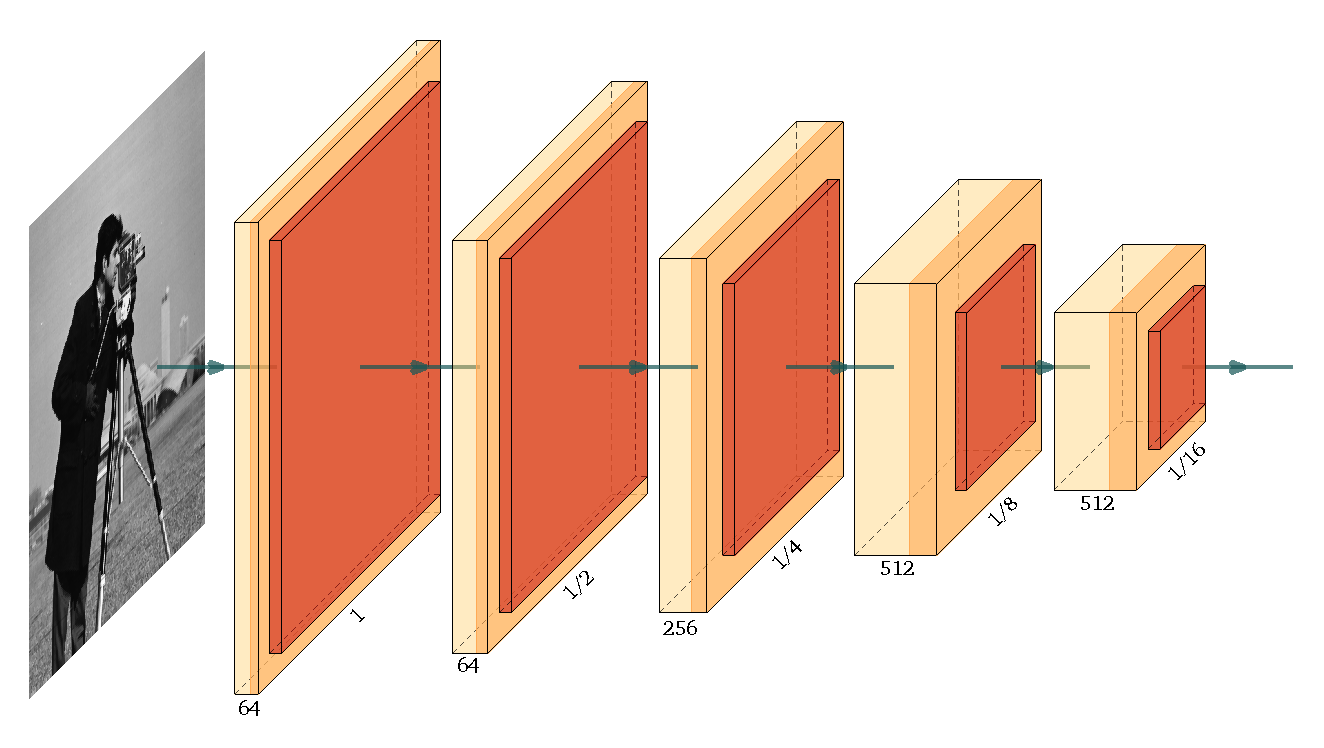
\includegraphics[width=0.7\textwidth]{figs/background/cnn-layers.pdf}
  \caption[Basic structure of a CNN]{The basic architecture of a CNN\@. The convolutions create stacks of feature maps (yellow) which are followed by an non-linear activation (orange), and the pooling layers (red) reduce the size of the feature maps. Here the pooling layer halves the spatial dimensions of the feature maps. Visualization library \parencite{haris_2018}.}\label{fig:back-cnn-example}
\end{figure}

A convolutional neural network consists of stacked and layered operations.
There are two types of layers, \textit{convolutional}, and \textit{spatial pooling}.
The convolutional layers extract \textit{feature maps} by applying several trainable filters to the input before applying a nonlinear activation function to the result.
The spatial pooling layers operate similarly by applying an operation to a receptive field moved over the input feature map.
The operation is designed to downsample the input, so the resulting feature map has reduced dimensions.
Figure~\ref{fig:back-cnn-example} shows an example of a simple CNN model; the convolutional layers control the depth of the activations while the pooling layers control their spatial dimensions.
The two layers are stacked alternatingly, with the idea that the complexity of the features extracted increases with the depth of the network.

\subsection{Convolution}
The central concept of the convolutional layer is the \textit{convolution operation}.
Let the kernel, \(w\), be a \(k\by k\) dimensional matrix.
This kernel will operate on the output of the preceding layer, \(x\).
The output from the convolution can be calculated as follows,

\[w\ast x_{ij}=\sum_{m}\sum_{n}  w_{mn}x_{i-m,j-n}\]

Where \((m,n)\) spans the index set of the kernel, which is center originated, i.e., \(w_{0,0}\) indexes the centroid of the kernel.
The patch of \(x\) involved in the sum at each step is referred to as the \textit{receptive field}.
As the operation is repeated for every index of \(x\), the receptive field slides across the input.
The resulting output of the convolution is referred to as a \textit{feature map}.

\begin{figure}[htb]
  \centering
  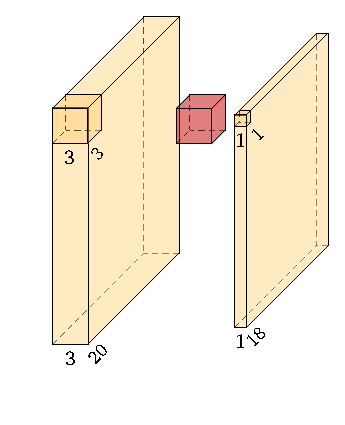
\includegraphics[width=0.4\textwidth]{figs/background/conv.pdf}
  \caption[Convolution operation]{Visualization of the convolution operation.
In red is a filter containing three \(3\by 3\) kernels.
The element wise multiplication between the filter and receptive field and subsequent summation produces a single scaler in the feature map.
The operation is repeated over the index set of the input, producing the complete feature map.}\label{fig:cnn}
\end{figure}

Usually, the input to a convolutional layer contains multiple channels, e.g.,\ an RGB input image with three channels representing the separate red, green, and blue color channels.
A stack of kernels is therefore used, one for each input channel.
Each channel is convolved with its kernel, and the result is added together across the channels, which produces a single feature map.
An example of such a convolution operation is shown in Figure~\ref{fig:cnn}.
This stack of kernels is referred to as a \textit{filter}.
For a convolutional layer to produce \(N\) feature maps, \(N\) filters are needed.
It is common to increase the number of filters as the image is continually downsampled through the layers on the neural network.

At the edges of \(x\) the sum is undefined because the receptive field moves beyond the bounds of \(x\), causing a reduction in the size of the output.
This can be mitigated by \textit{padding} the input.
When the receptive field moves beyond the bounds of \(x\), a stand-in value is used instead.
This can be visualized as \textit{padding} the input with said value.
Zero is often used as the padding value.

Dimensionality reduction is also possible using the concept of \textit{stride}, which refers to how the receptive field moves across the input relative to the index of the feature map.
In the base case, the receptive field moves by one step for every element in the feature map.
With an increased stride, the receptive field `jumps over' positions for every step in the feature map, thus shrinking its size.

One of the more essential aspects of convolutions arises from the fact that the kernel is applied in the same way over the whole image.
This parameter sharing means that features are extracted from the input, regardless of their location\ \parencite{lecum1989}.
It also reduces the computational complexity involved in training the model.

Because convolution is a linear operation, non-linearity must be added if the network is to be able to approximate a nonlinear function.
As with regular fully connected networks, this is achieved by applying an activation function to the feature map.
The same activation functions that are commonly used in fully connected networks are also used in CNNs.
Because of the depth of the models’ architectures in use today, the \textit{rectified linear unit} (ReLU), and its variations, are commonly used.

\subsection{Spatial pooling}
Even though the convolution operation extracts features wherever they exist within an image, a new problem arises when layers are stacked to extract higher-level features from the combination of features below.
Local variations in the relative placement of features will significantly impact later filters' ability to combine them. This would have to be accounted for by dramatically increasing the number of filters.\ \textcite{lecun1998gradient} presents a simple solution to this problem with a \textit{sub-sampling} layer, referred to as a \textit{pooling} layer today, which reduces the dimensions of the feature map by applying a local pooling function, similarly to the convolution operation.
Standard pooling functions are maximum and average.
The pooling operation is applied to each channel separately, so only the width and height are downsampled.
Pooling retains the relative placement of features within the image while allowing the network to ignore smaller variations in the relative configuration of features across all the channels of the feature map.

\subsection{Cross channel pooling}
As mentioned, it is customary to increase the depth of the feature maps as they get downsampled throughout the network.
This is necessary if the model is to learn more complex features that may require many layers to be represented in full.
Combining information from multiple channels could help build more rich feature maps.
This is the proposal in\ \textcite{lin2014network}.
To enhance model discriminability, they propose a `Network in Network', a fully connected layer working across the channels.
This effectively creates connections between local features across the channels of the feature maps, as shown in Figure~\ref{fig:back-cross-channel}.

\begin{figure}[htbp]
  \centering
  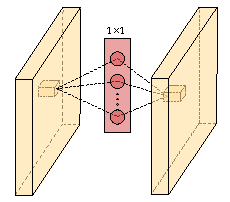
\includegraphics[width=0.4\textwidth]{figs/background/cross-channel.pdf}
  \caption[Cross channel pooling architecture]{Visualization of a cross channel pooling architecture.This simple example models a single fully connected layer using a \(1\by 1\) convolution.}\label{fig:back-cross-channel}
\end{figure}

The technique is however most commonly used as an optimization that removes computational bottlenecks in deeper networks \parencite{szegedy2014going}.
By placing a \(1\by 1\) convolution with reduced output depth in front of a larger \(3\by 3\) or \(5\by 5\) convolution, the computational cost is reduced, which allows for much deeper networks. For instance, given an input depth of 500, a \(3\by 3 \by 500\) convolution requires 2,250,000 parameters, but if a \(1\by 1 \by 250\) is used first, the total number of parameters in both layers is only 1,250,000.
The technique is now commonplace and featured in all deep CNN architectures.

\subsection{Batch normalization}
As the network trains, the parameters in each layer change. This causes the distribution of each layer’s output to shift.
As the distribution from previous layers changes, this shift is propagated through to the layers downstream, and so each layer must deal with ever-changing input distributions.
To overcome this, lower learning rates and careful parameter initialization is required.

A much more effective solution has been proposed by\ \textcite{ioffe2015batch} called \textit{Batch Normalization} (BN).
The proposed solution for convolutional networks is to normalize the layers from each convolution independently. Given a layer activation with \(d\) feature maps \(\mathbf{a}=\left(a^{(1)},\dots,a^{(d)}\right)\), each feature map \((k)\) is normalized (pre activation) as follows,

\begin{equation*}
  \widehat{a}^{(k)}=\frac{a^{(k)}-\mean{a^{(k)}}}{\sqrt{\var{a^{(k)}}}}
\end{equation*}

where \(\var{\cdot}\) and \(\mean{\cdot}\) are respectively the batch variance and batch mean over both the mini-batch and spacial locations of the feature map, thus maintaining the convolutional property of spatial invariance within feature maps.
However, this normalization could be undesirable in certain circumstances.
For instance, if the inputs of a ReLU activation are normalized, roughly half of the features will be truncated at 0.
To account for this, the normalized values are scaled and shifted before activation.
Two parameters, \(\gamma^{(k)}\) and \(\beta^{(k)}\) are introduced for each feature map, and the normalized values are scaled and shifted as follows,

\begin{equation*}
  y^{(k)}=\gamma^{(k)}\,\widehat{a}^{(k)}+\beta^{(k)}
\end{equation*}

The parameters are learned together with the original filters and restore the representative power of the layers.
By allowing the filters to only focus on learning features, instead of adapting to constantly shifting input distributions, training is accelerated, allowing for higher learning rates.

\subsection{Data augmentation}
Deep learning in general, and deep convolutional networks in particular, require a large amount of data to generalize to a solution properly.
Data augmentation is a technique whereby the size of a dataset is artificially increased by applying transformations to the existing data.
This has been an important regularization technique and a critical component of many established models, such as ResNet\ \parencite{he2015deep} and AlexNet\ \parencite{alexnet}.
It is argued by\ \citeauthor{Hern_ndez_Garc_a_2018} that data augmentation alone is more beneficial to training than using explicit regularization such as dropout or weight decay \parencite{Hern_ndez_Garc_a_2018}.

Many different transformations can be applied to image data. Lighter augmentations include flipping an image either horizontally or vertically or translating the image by some vector. Heavier augmentations include more affine transformations, such as rotating, sheering, scaling the image, or adjusting the image's contrast, brightness, and hue.

Augmentations are limited only by the fact that they must preserve the necessary information that the model needs to make a prediction and by the computational cost they impose on the training procedure. In object detection, augmentations must also transform the ground truth labels, which also incurs additional costs.

\subsection{Transfer learning}
A different approach to solving for small datasets is the concept of \textit{transfer learning}.
There is a generally accepted assumption in machine learning that the training and testing data must be sampled from the same distribution and share the same feature space. Transfer learning challenges this assumption \parencite{pan_yang_2010}.
A successful knowledge transfer can lead to a better generalization in a new domain with less data by training a model for one task in a domain with an abundance of data.

Transfer learning is widely used in the models presented in Chapter~\ref{cha:related}, both those used in pollen classification and general object detection.
The source is usually an image classification model trained on a large dataset, such as the previously mentioned ResNet and AlexNet architectures.
With object detection systems, the pre-trained model functions as a feature extractor for the detection architecture.
In the domain of pollen classification, transfer learning has been shown to improve accuracy in CNN based classifiers, even though the source and target domain are vastly different.

\section{Recurrent Neural Networks}\label{sec:back-rnn}
Recurrent neural networks are not a major part of this thesis, but are used closely related work, so understanding the basic workings of this class of neural networks is needed.

A recurrent neural network is a special type of network used to process sequences of information, e.g., signals, text, or time-series.
It adds \textit{working memory} to the layers such that the activation of previous elements in a sequence are `remembered'.
Given an input sequence \(\mathbf{X}=\{x^1,\dots,x^n\} \), each element is activated in turn, but when processing element \(x^n\), the activation of \(x^{n-1}\) is added.

\section{Metrics}\label{sec:back-metrics}
An essential step towards building a model is defining how to measure its performance.
Implicitly, this is done through the construction of a \textit{Loss function}.
The models examined in this thesis do not employ novel Loss functions, so delving into their construction is not warranted.
The metrics used when measuring the performance of object detectors, specifically, are nonetheless of interest.

Object detection is a multi-task problem incorporating both the localization and classification of objects.
Throughout this thesis, when referring to a \textit{detection} made by an object detection system, this refers to a proposed boundary that the system believes encloses an object of a particular class.
Every detection encodes both localization and a class label.
A correct detection refers to a detection that matches a ground truth, i.e., a predicted boundary with a particular class matches that of a ground truth of the same class.

\subsection{Precision and recall}
The precision and recall of a model refer to its ability to correctly locate and label the objects within an image.
Before defining precision and recall, the following quantities must be introduced,

\begin{center}
  {\setlength{\fboxsep}{1em}
  \fbox{%
  \begin{minipage}{0.9\textwidth}
  {\bf True Positive (TP):} Number of objects correctly located and labelled.\\[1ex]
  {\bf False Positive (FP):} Number of incorrect predictions.\\[1ex]
  {\bf True Negative (TN):} Correct non-prediction, not usually relevant.\\[1ex]
  {\bf False Negative (FN):} Number of objects missed by model.
  \end{minipage}}}
\end{center}

Precision measures the model's accuracy, i.e.,~how many of the positive predictions are correct.
Recall measures how many of the positive instances the model correctly labels.
They are computed from the above quantities as follows,

\begin{align*}
  \text{\bf precision}=\frac{TP}{TP+FP}\\[1em]
  \text{\bf recall}=\frac{TP}{TP+FN}
\end{align*}

These two metrics are the basis for how all object detection models are evaluated, and there is usually a tradeoff between the two.
For instance, a model can have a very high recall, meaning it correctly identifies most potential objects, but the precision is reduced if it also identifies many other non-objects.
Inversely, a model could be sure that it returns correctly identified objects at the cost of ignoring objects it is unsure about.

A popular accuracy measure that derives from the precision and recall values is the \(F_1\) score, and it may also be referred to as the dice score.
It is defined as follows,
%
\begin{align*}
  F_1=2\frac{\text{precision}\cdot\text{recall}}{\text{precision}+\text{recall}}
\end{align*}

The \(F_1\) score measures the balance between precision and recall values and is useful in cases where both measures are \textit{equally} important performance indicators.

\subsection{Intersection over union}
The correctness of a detection has been defined as `a detection that matches a ground truth'.
Classification has a simple binary solution; two classes are either the same or different.
A positive solution to a binary localization problem would require pixel-perfect similarity between the predicted boundary and ground truth, which would be an extremely high bar to clear.
For a more lenient approach, one could instead assign a \textit{localization score} to the predicted boundary based on how well it matches the ground truth.
A positive solution could then be defined as a boundary with a localization score above some threshold.

Most object detection systems use \textit{intersection over union} (IoU) to score the match between boundaries.
As the name indicates, it is defined as the ratio between the intersection and union of two boundaries,

\begin{figure}[htb]
  \centering
  \begin{gather*}
    \text{IoU}=\frac{\text{area of intersection}}{\text{area of union}}
  \end{gather*}
  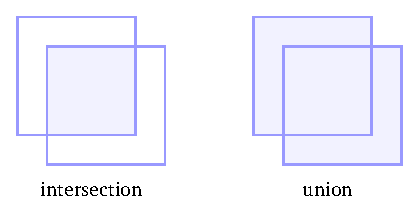
\includegraphics[width=0.55\textwidth]{figs/background/iou.pdf}
\caption[Intersection over union]{Visualization of the intersection over union of two boundaries.
The named region is shaded.}\label{fig:iou}
\end{figure}

The definition of what is considered a correct prediction (TP) can then be defined.
Given prediction \(\hat{X}\) with label \(\hat{X}_l\) and bounding box \(\hat{X}_u\). \(\hat{X}\) is considered a True Positive if there exists a ground truth \(Y\), where \(Y_{l}=\hat{X}_l\) and \(\text{IoU}(\hat{X}_u, Y_{u})\ge \mu \).
Where \( \mu \) is some threshold value, often 0.5.

\subsection{Mean average precision}
Mean average precision (mAP) is a popular metric for measuring the performance of object detection models.
It is computed by taking the mean of the \textit{average precision} values for each class.

From a list of all detections made for a class, ranked in ascending order of confidence, each is labeled either true positive or false negative.
In cases where multiple predictions match the same ground truth, only the highest-ranking prediction is considered a true positive.
The cumulative precision and recall are computed from the ordered list of predictions, and from these values, a precision-recall curve is drawn.
This shows how precision changes as recall rises over the range [0,1] as more and more detections from the ranked list are included in the precision/recall calculations.
The AP describes the shape of the precision-recall curve and can be calculated in a few different ways.
This thesis will use the definition of AP specified in the evaluation procedure for the VOC2007 image detection challenge.
For convenience, the definition of AP, as given in\ \textcite{everingham2010pascal} is repeated below.

AP is measured by taking the mean of precision values taken at 11 evenly spaced recall values as follows,

\begin{equation}\label{eq:average-precision}
  AP=\frac{1}{11} \sum_{r\in \{0,0.1,\dots,1\}}p_{interp}(r)
\end{equation}

Because the precision-recall curve often times is quite erratic, the precision value at a given recall level, \(r\), is interpolated by finding the maximum precision value at any recall level exceeding \(r\),

\begin{equation*}
  p_{interp}(r)=\max_{\tilde{r}:\tilde{r}\geq r}p(\tilde{r})
\end{equation*}

This section has detailed the current methods employed for automated pollen counting and the foundational building blocks of a CNN\@.
Most research and application of CNN based methods is regarding classification, which only solves part of the problem of counting pollen.
A subcategory of deep CNNs capable of predicting both classes and locations is required to automate the task fully.
The next chapter will detail how \textit{object detection} can be solved using a CNN by detailing how they have been used to solve tasks similar to pollen counting.
The available literature relating to other attempts at solving the problem of counting pollen will also be given.
